\subsection{Расстояние и размеры}
\term{Астрономическая единица}~--- единица измерения расстояния в астрономии, 
равная большой полуоси орбиты Земли.\begin{equation}
	1~\au = 149\:597\:870\:700~\text{м} \simeq 1.5 \times 10^{11}~\text{м}.
\end{equation}

\term{Годичный параллакс} ($\pi$) объекта~--- это угол, под которым видно 
орбиту Земли из окрестностей данного объекта. Применяется к объектам вне 
Солнечной системы. \begin{equation}
	\tg \pi = \frac{a_\oplus}{r},
	\label{eq:parallax-sin}	
\end{equation}
где $a_\oplus$~--- большая полуось орбиты Земли и $r$~--- расстояние до объекта 
имеют одинаковые единицы измерений. Учитывая малость угла $\pi$, можно считать $\tg\pi \simeq \pi$ в \eqref{eq:parallax-sin}, тогда
\begin{equation}
	\pi = \frac{a_\oplus}{r}.
	\label{eq:parallax}
\end{equation} 
\begin{figure}[h!]
	\centering
	\vspace{-1pc}
	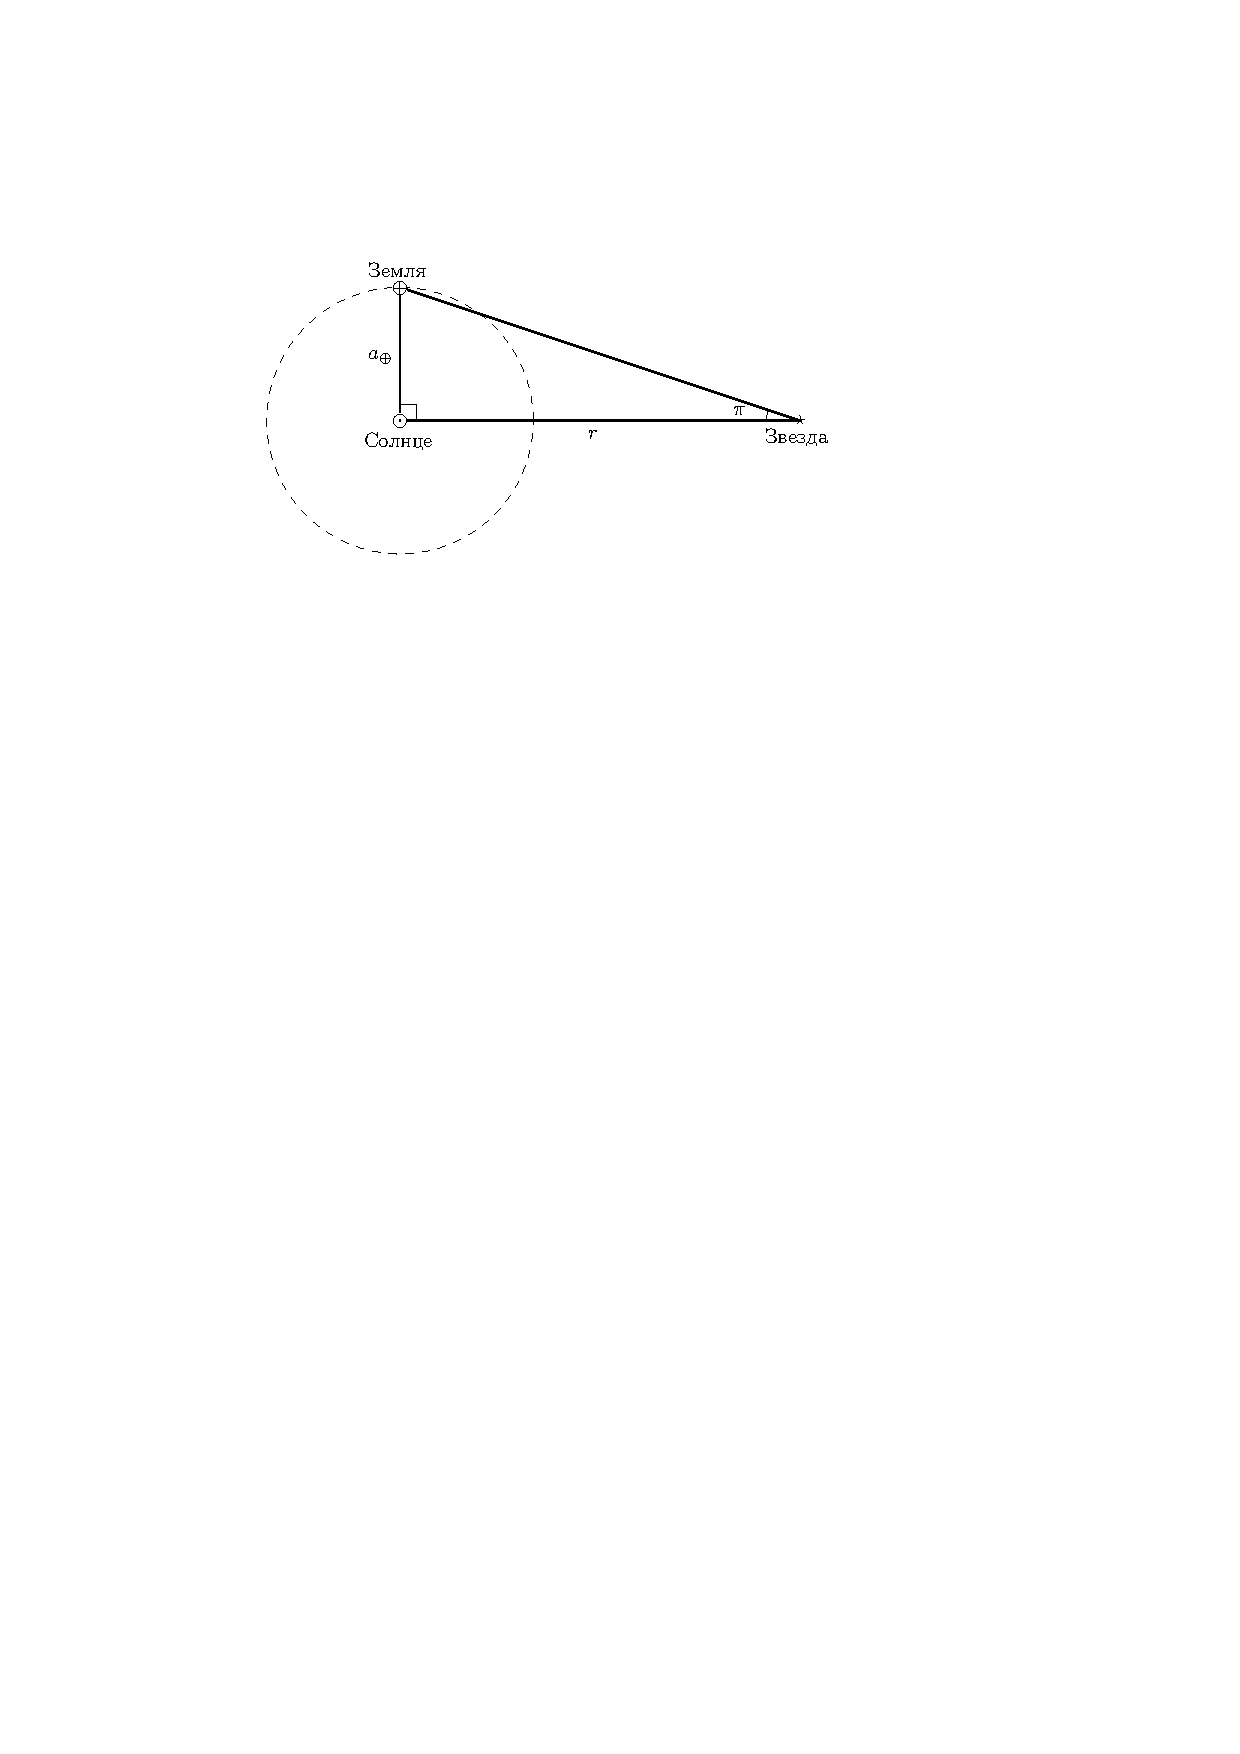
\includegraphics[width = 0.7\tw]{parallax.pdf}
	\caption{Схема годичного параллакса}
\end{figure}

Расстояние $r$, с которого большая полуось орбиты Земли $a_\oplus$ видна под углом $\pi = 1''$ называется \term{1 парсеком}. Так как \begin{equation}
	1~\text{рад} = \frac{180^\circ}{\pi} \simeq  3 438' \simeq 206265'' 
\quad \Longrightarrow \quad \mathsf{1~\text{\sffamily пк} = 
206265~\text{\sffamily а.\,е.}},
\end{equation} 
следовательно, записывая большую полуось орбиты Земли в \au, а расстояние до звезды в парсеках, получаем параллакс в секундах. Таким образом,
\begin{equation}
	r_\text{пк} = \frac{1~\au}{\pi''}.
\end{equation}

\term{Угловой размер объекта}~--- это угол, под которым видно объект. Для сферически симметричных объектов с радиусом $R$, угловой размер (диаметр) при наблюдении с расстояния $r$ определяется как
\begin{equation}
\rho = 2 \arcsin \frac{R}{r}.
\end{equation}
В случае, когда $r\gg R$, можно считать, что $\sin \rho \simeq \rho$, тогда
\begin{equation}
	\rho \simeq \frac{2 R}{r}.
\end{equation}

\vspace{-1.5pc}
\begin{figure}[h!]
	\begin{minipage}[b]{0.5\tw}
		\begin{flushleft}
			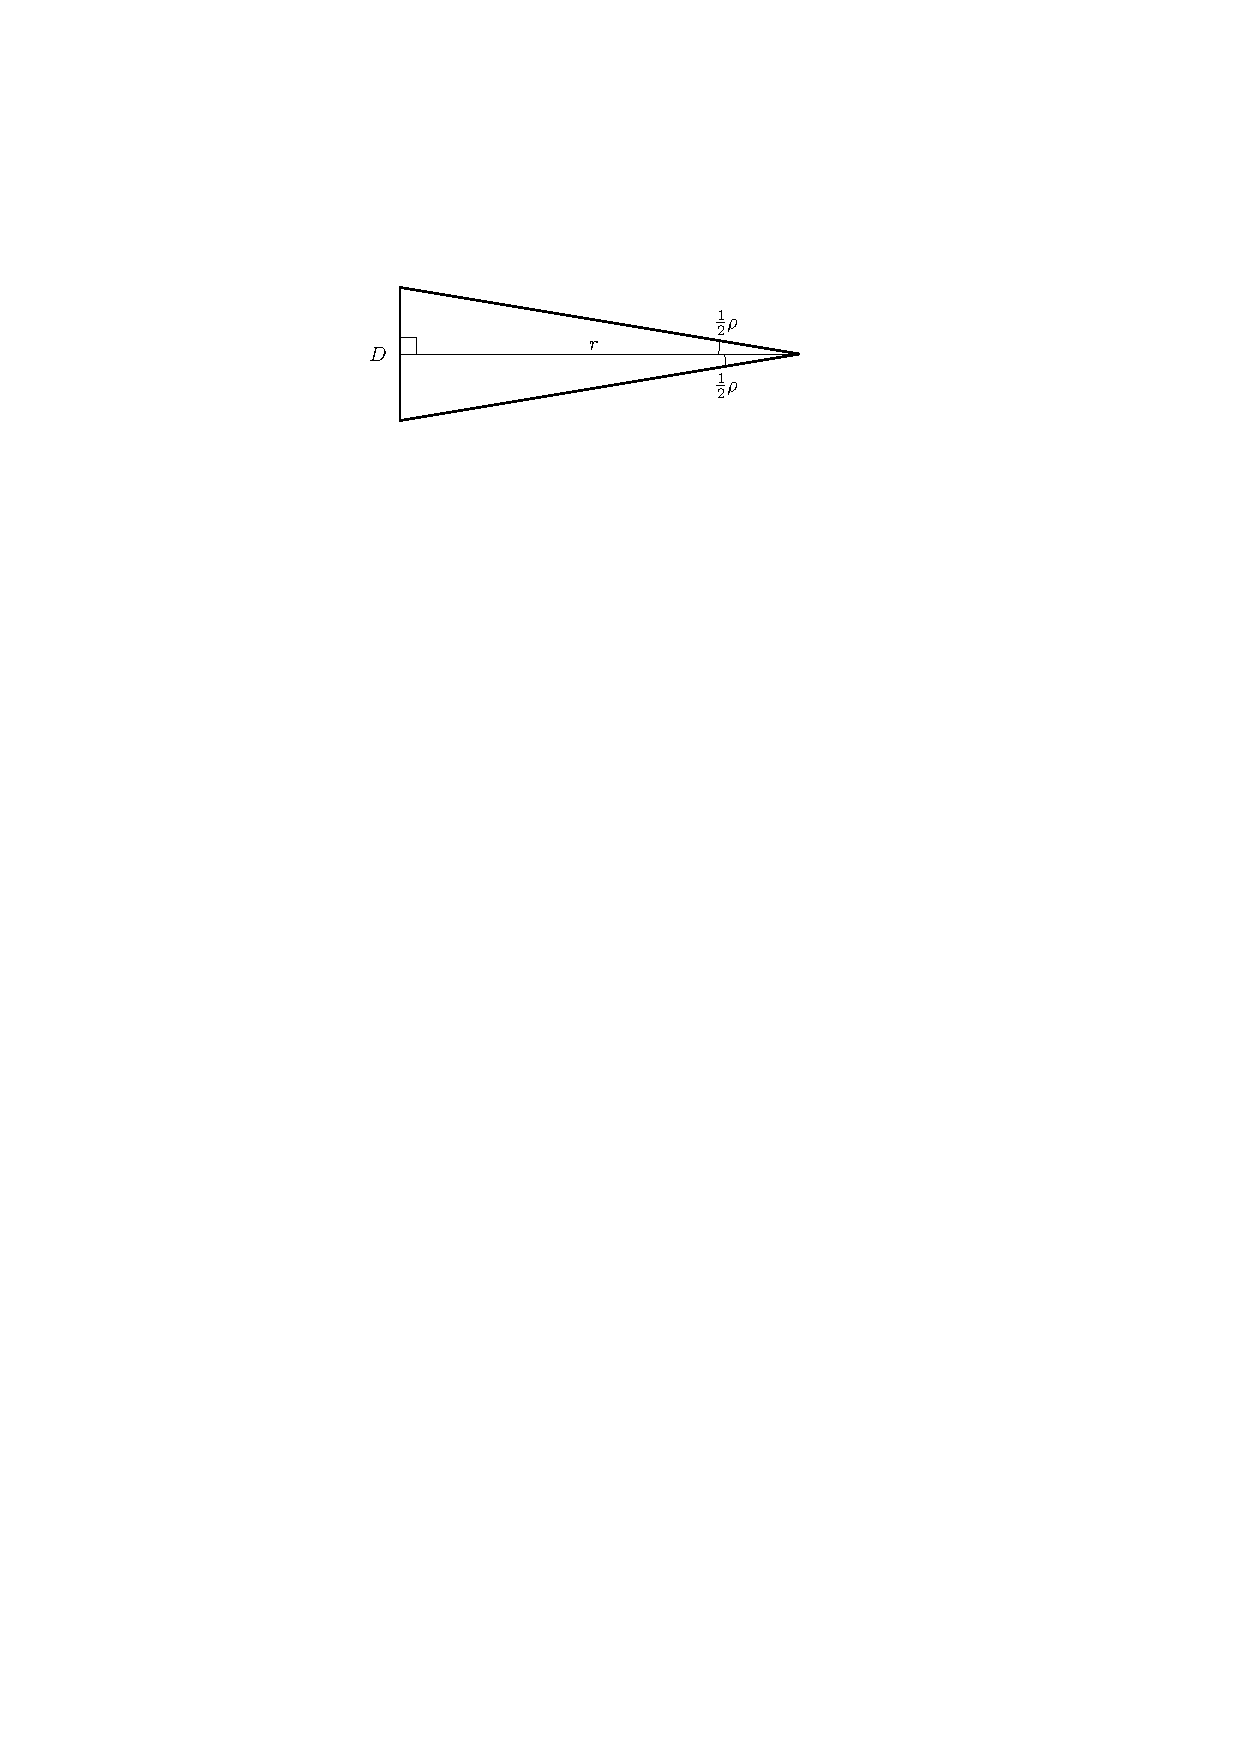
\includegraphics[width = 0.93\tw]{angle-size}
			\captionof{figure}{Угловой размер}
		\end{flushleft}
	\end{minipage}
	\begin{minipage}[b]{0.5\tw}
		\centering
		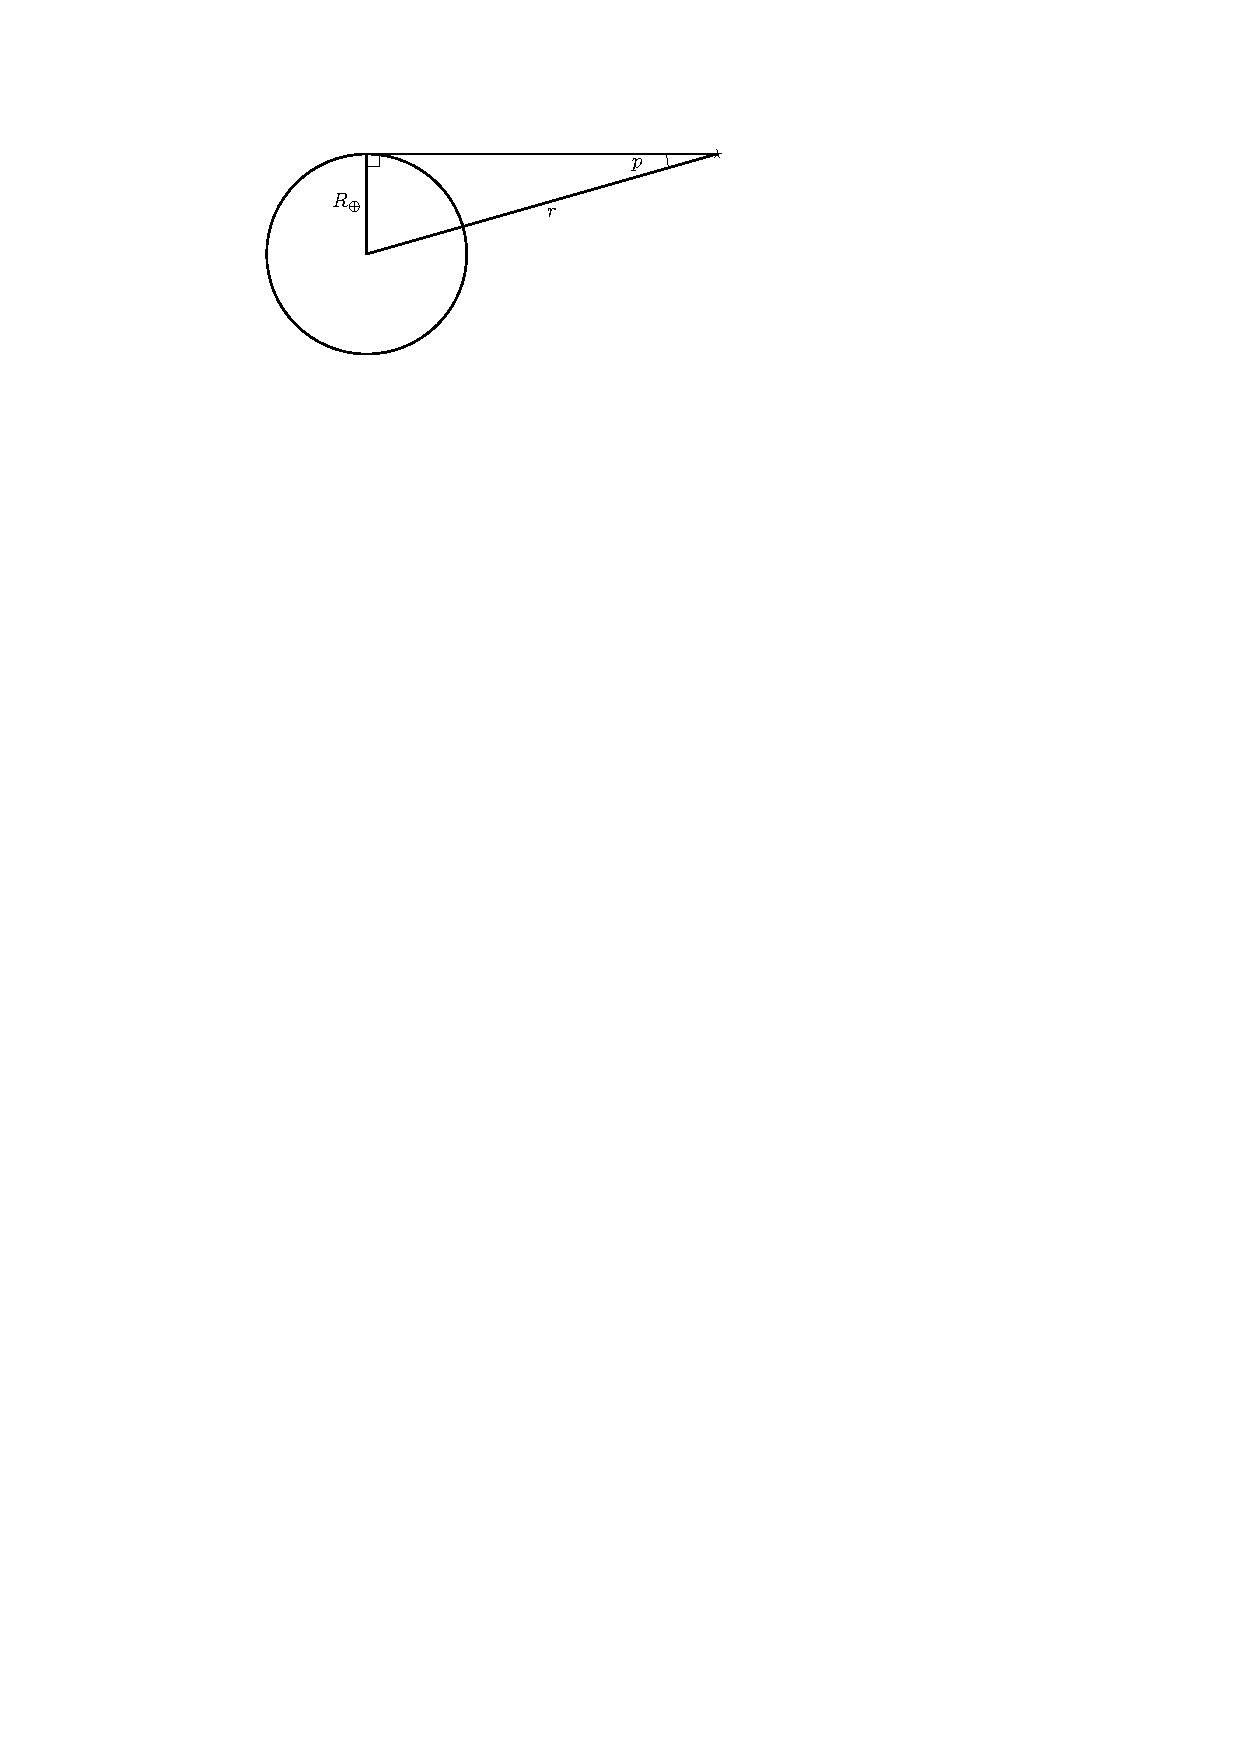
\includegraphics[width = \tw]{parallax-horiz}
		\captionof{figure}{Горизонтальный параллакс}
	\end{minipage}
\end{figure}

\term{Горизонтальный параллакс}~$(p)$~--- это угол, под которым виден радиус Земли~$R_\oplus$ для наблюдателя в центре объекта, когда последний находится на горизонте:
\begin{equation}
\sin p=\frac{R_\oplus}{r}.
\end{equation}

\term{Правило Тициуса-Боде} --- эмпирическая формула, приблизительно описывающая 
радиусы орбит планет в Солнечной системе:
\begin{equation}r=\frac{3\cdot 2^n+4}{10}, \quad n=-\infty, 0, 1, 2...
\end{equation}

